We calculate this for the periodic flow case in the next section of \tty{viz.ipynb}.
We begin by computing both sides of the Bernoulli relationship in the base case as a sanity check for the method.
Using the quantities $p_0$, and $u_0$ at $x=0$ (start of the channel) we find an energy density of 0.339.
Using the quantities $p_i$ and $u_i$ at $x=100$ (center of the channel) we find an energy density of 0.334.
Since we expect these to be approximately equal, it's encouraging that they are this close together.
In the Python function \tty{calc\_pressure\_narrow} we calculate the pressure $p_i$ that would be implied
at the narrowest point of the channel by solving this relationship for $p_i$ in terms of $p_0$, $u_0$ and $u_1$.

\begin{figure}[H]
    \centering
    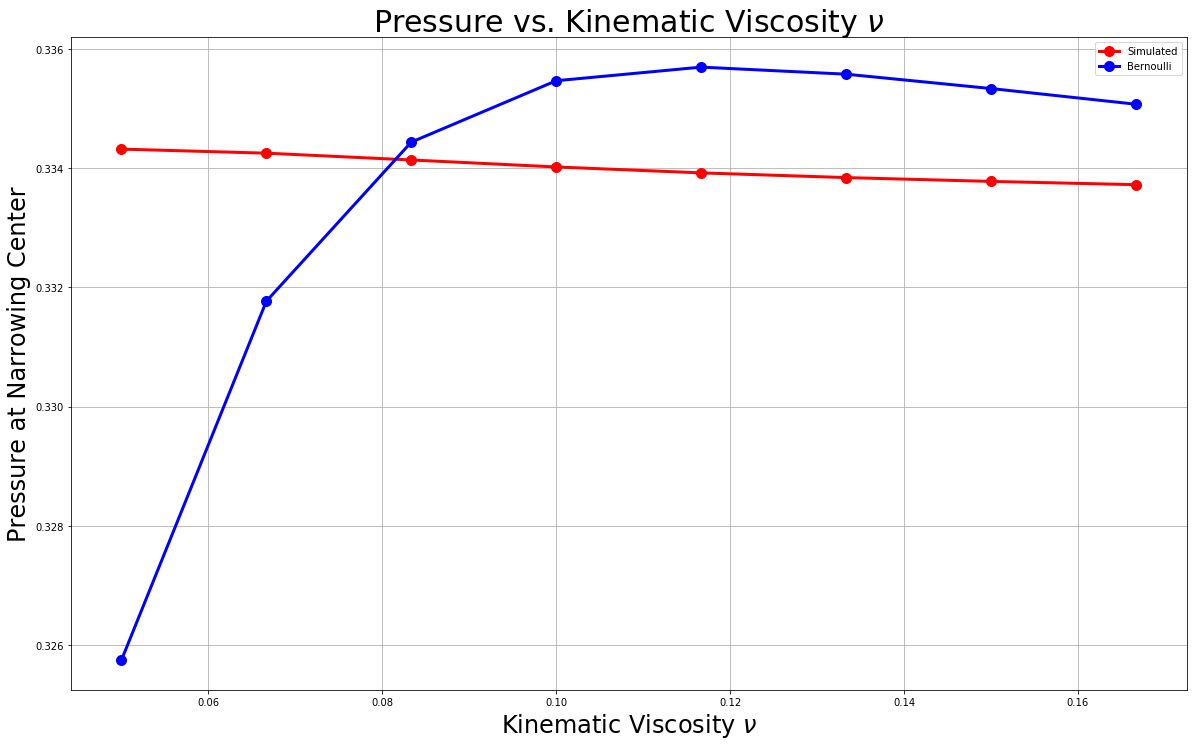
\includegraphics[width=0.85\textwidth]{lbm_pbc_pressure_vs_nu.png}
    \caption{Pressure vs. the Bernoulli estimate of the periodic channel.}
\end{figure}

The scale on this plot is very compressed, so it's important not to overreact to the shape of the curves being different.
The high level story here is the pressure scale ranges from 0.326 to 0.336, so the two methods are actually
in quite good agreement over this range of viscosities.
One thing the chart does seem to be suggesting is that that the Bernoulli approximation is breaking down at an
accelerating rate as the viscosity drops in the range of 0.05.
This isn't too surprising, when we recall that it's an ``inviscid'' approximation.
That approximation will be more accurate at higher viscosities.